\documentclass[11pt]{article}

% ---------- packages ----------
\usepackage[utf8]{inputenc}
\usepackage[T1]{fontenc}
\usepackage[margin=1in]{geometry}
\usepackage{amsmath,amssymb}
\usepackage{graphicx}
\usepackage{booktabs}
\usepackage{array}
\usepackage{caption}
\usepackage{xcolor}
\usepackage{enumitem}
\usepackage{tikz}
\usetikzlibrary{positioning,arrows.meta,fit}
\usepackage[section]{placeins}
\usepackage[colorlinks=true,linkcolor=blue,urlcolor=blue,citecolor=blue]{hyperref}

\graphicspath{{stage2/results/figures/}{./}}
\newcommand{\code}[1]{\texttt{#1}}

% Bold-red flag: a result currently established ONLY on the DDSM (second) dataset,
% for which a CovidGAN counterpart still needs to be run.
\newcommand{\ddsmonly}[1]{\textcolor{red}{\textbf{#1}}}

% ---------- title ----------
\title{\textbf{Reproducing, Diagnosing, and Rescuing the CovidGAN Claim}\\[2pt]
\large --- Validated on a Second Dataset (Condensed) ---\\[6pt]
\normalsize Final Project, Part 2 --- Joint Report}
\author{Hila Fishman \and Maya Hayat}
\date{}

\begin{document}
\maketitle
\vspace{-2.0em}

\noindent
Reconstruction, diagnosis, and improvement of Waheed et al., \emph{``CovidGAN: Data
Augmentation Using Auxiliary Classifier GAN for Improved Covid-19 Detection''}, IEEE
Access, vol.~8, 2020.

\medskip
\noindent\textbf{Overview.} We reconstruct the paper's AC-GAN + VGG16 COVID-19
detector and find that its central claim --- a \textbf{+10-point accuracy lift} from
GAN augmentation --- \textbf{does not reproduce} (§\ref{sec:recon}). The rest of the
report diagnoses \emph{why} and fixes it (§\ref{sec:improvedarch}--§\ref{sec:results}),
and --- to check that the failure is not just an artifact of our particular COVID
dataset --- \textbf{re-runs the same pipeline on a second dataset} (CBIS-DDSM
mammography), reporting the DDSM result alongside each main CovidGAN claim. A result
currently established \emph{only} on DDSM (still awaiting a CovidGAN counterpart) is
flagged like \ddsmonly{this}. CovidGAN is the primary dataset and leads every
experiment; DDSM numbers are from Weights~\&~Biases
(\code{maya-hayat-ariel-university/ddsm-acgan}).

% =====================================================================
\section{Original architecture}
\label{sec:arch}
% =====================================================================
The pipeline has two models: an \textbf{AC-GAN} that synthesizes chest-X-ray (CXR)
images and a \textbf{VGG16-based classifier} that detects COVID-19; synthetic images
augment the classifier's training set (Figure~\ref{fig:arch}).

\begin{figure}[htbp]
\centering
\tikzset{
  b/.style={draw,rounded corners,minimum height=7mm,minimum width=14mm,font=\scriptsize,align=center,fill=blue!8},
  io/.style={draw,rounded corners,minimum height=7mm,minimum width=12mm,font=\scriptsize,align=center,fill=black!8},
  frz/.style={draw,rounded corners,minimum height=7mm,minimum width=14mm,font=\scriptsize,align=center,fill=black!18},
}
\textbf{(a) AC-GAN generator}\\[2pt]
\resizebox{\textwidth}{!}{%
\begin{tikzpicture}[>=Latex,node distance=4mm and 6mm]
  \node[io] (z) {noise $z$\\$\mathbb{R}^{100}$};
  \node[io,below=of z] (c) {label $c$};
  \node[b,right=of z] (zd) {Dense+ReLU\\$7{\times}7{\times}1024$};
  \node[b,right=of c] (cd) {Embed$\to$Dense\\$7{\times}7{\times}1$};
  \node[b,right=7mm of zd] (cat) {concat\\$7{\times}7{\times}1025$};
  \node[b,right=of cat] (u1) {TConv$\uparrow$\\$14^2$};
  \node[b,right=of u1] (u2) {TConv$\uparrow$\\$28^2$};
  \node[b,right=of u2] (u3) {TConv$\uparrow$\\$56^2$};
  \node[b,right=of u3] (u4) {TConv+tanh\\$112^2$};
  \node[io,right=of u4] (img) {image\\$112^2{\times}3$};
  \draw[->] (z) -- (zd); \draw[->] (c) -- (cd);
  \draw[->] (zd) -- (cat); \draw[->] (cd) -- (cat);
  \draw[->] (cat) -- (u1); \draw[->] (u1) -- (u2); \draw[->] (u2) -- (u3);
  \draw[->] (u3) -- (u4); \draw[->] (u4) -- (img);
\end{tikzpicture}}\\[8pt]
\textbf{(b) AC-GAN discriminator}\hspace{2mm}\textbf{(c) VGG16 detector}\\[2pt]
\resizebox{\textwidth}{!}{%
\begin{tikzpicture}[>=Latex,node distance=4mm and 6mm]
  \node[io] (img) {image};
  \node[b,right=of img] (d5) {5 conv$\downarrow$\\$7{\times}7{\times}512$};
  \node[b,above right=2mm and 7mm of d5,fill=green!10] (val) {validity\\(real/fake)};
  \node[b,below right=2mm and 7mm of d5,fill=orange!12] (cls) {class\\(COVID/Normal)};
  \draw[->] (img) -- (d5); \draw[->] (d5) -- (val); \draw[->] (d5) -- (cls);
  \node[io,right=22mm of val] (im2) {image};
  \node[frz,right=of im2] (vgg) {VGG16 base\\\textit{frozen}};
  \node[b,right=of vgg] (gap) {GAP+Dense(64)\\Dropout};
  \node[b,right=of gap] (o2) {Dense(2)\\softmax};
  \draw[->] (im2) -- (vgg); \draw[->] (vgg) -- (gap); \draw[->] (gap) -- (o2);
\end{tikzpicture}}
\caption{\textbf{(a)}~Generator fuses noise + label and upsamples $7{\to}112$ through
four transpose-conv blocks ($\sim$22M params). \textbf{(b)}~Discriminator downsamples
to $7{\times}7{\times}512$ and splits into the two AC-GAN heads ($\sim$2M).
\textbf{(c)}~Detector is a \emph{frozen} ImageNet VGG16 + small head --- only
$\sim$33K of $\sim$14.7M params train, per the paper.}
\label{fig:arch}
\end{figure}

\noindent\textbf{Losses / hyperparameters.} GAN objective: \code{BCEWithLogits}
(validity) + \code{CrossEntropy} (class) for both $D$ and $G$, one-sided label
smoothing (real target 0.9); classifier: \code{CrossEntropy}. GAN trained batch~64,
Adam \code{lr=2e-4}, $\beta_1{=}0.5$, \textbf{2000 epochs}; classifier batch~16,
Adam \code{lr=1e-3}, images $112{\times}112$. Paper split: train COVID/Normal
331/601, \textbf{test 72/120 (192)}.

% =====================================================================
\section{Paper results (the target)}
% =====================================================================
Accuracy on the held-out 192-image real test set, in two configurations reused
throughout: \textbf{CNN-AD} (real data only) and \textbf{CNN-SA} (real + synthetic).

\begin{table}[htbp]\centering
\begin{tabular}{@{}lc@{}}\toprule
\textbf{Configuration} & \textbf{Accuracy} \\ \midrule
CNN-AD (real only) & \textbf{85\%} \\
CNN-SA (+ synthetic) & \textbf{95\%} \\ \bottomrule
\end{tabular}\end{table}

\noindent The claim under test is the \textbf{+10-point} lift (CNN-SA $-$ CNN-AD),
concentrated in COVID recall. \emph{Metrics:} \textbf{accuracy} (paper's) =
correct/total on real test; \textbf{recall} = TP/(TP+FN) per class (the clinically
meaningful axis, studied in class); \textbf{FID} (studied in class) judges
\emph{generator} realism (lower~=~better); a \textbf{transfer probe} (train on
synthetic alone, test on real) judges whether synthetic carries real class signal. A
recurring finding: none of these generator-side measures predicts downstream value.

% =====================================================================
\section{Reconstruction results --- the claim does not reproduce}
\label{sec:recon}
% =====================================================================
We reimplemented the pipeline in PyTorch, trained the GAN for the paper's 2000
epochs, generated a synthetic pool (1669 COVID + 1399 Normal), and evaluated on the
192-image real test set.

\begin{table}[htbp]\centering
\begin{tabular}{@{}lcc@{}}\toprule
\textbf{Configuration} & \textbf{Paper} & \textbf{Our reconstruction} \\ \midrule
CNN-AD (real only)   & 85.00\% & \textbf{90.62\%} \\
CNN-SA (+ synthetic) & 95.00\% & \textbf{90.10\%} \\
Augmentation lift    & +10.00  & \textbf{$-$0.52 (flat)} \\ \bottomrule
\end{tabular}\end{table}

\noindent Two anomalies: \textbf{(A)} our baseline is \emph{higher} than the paper's
(90.6\% vs 85\%), and \textbf{(B)} augmentation is \textbf{flat}, not +10. We ruled
out the trivial explanations and then diagnosed each.

\paragraph{Not a bug, not a data-pipeline error.} A layer-by-layer audit confirms the
reconstruction matches the paper (VGG16 frozen, only $\sim$33K trainable params) ---
so the anomalies are not an implementation bug --- and we verified the dataset
pipeline itself is correct (right sources, de-duplication, and the paper's 331/601
train, 72/120 test split) --- so they are not a data-loading error either.

\paragraph{Anomaly A --- why the baseline is higher.} Our working hypothesis is that
the \textbf{data available today is cleaner and more separable} than the paper's 2020
hand-merged set: the modern Kaggle CXR database has been re-released several times and
the authors published no manifest of their exact selection, so their original set is
\emph{not reproducible}. Crucially, matching only the \emph{number} of images
(403/721) is \textbf{not enough} --- the images themselves are easier --- so our
detector does legitimate but easier classification (COVID recall 0.69$\to$0.89), with
no room for a +10 gain.

\paragraph{Anomaly B --- why augmentation is flat.} Two diagnostics:
\begin{itemize}[nosep,leftmargin=1.4em]
  \item \textbf{The synthetic pool carries no transferable pathology.} A classifier
        trained on the synthetic pool \emph{alone} scores \textbf{55.2\%} on real test
        (COVID recall 0.22) --- \emph{below} the 62.5\% majority floor. The AC-GAN
        stamped an easy class-conditioned \textbf{``fingerprint''} (a global
        brightness style; plainly visible in Figure~\ref{fig:samples}), not real
        pathology.
  \item \textbf{Image quality is not the cap.} FID roughly \emph{halved} from the
        25-epoch to the 2000-epoch generator (504.4$\to$272.7) with \emph{no}
        downstream change --- so generation quality is not what limits augmentation.
\end{itemize}

\begin{figure}[htbp]\centering
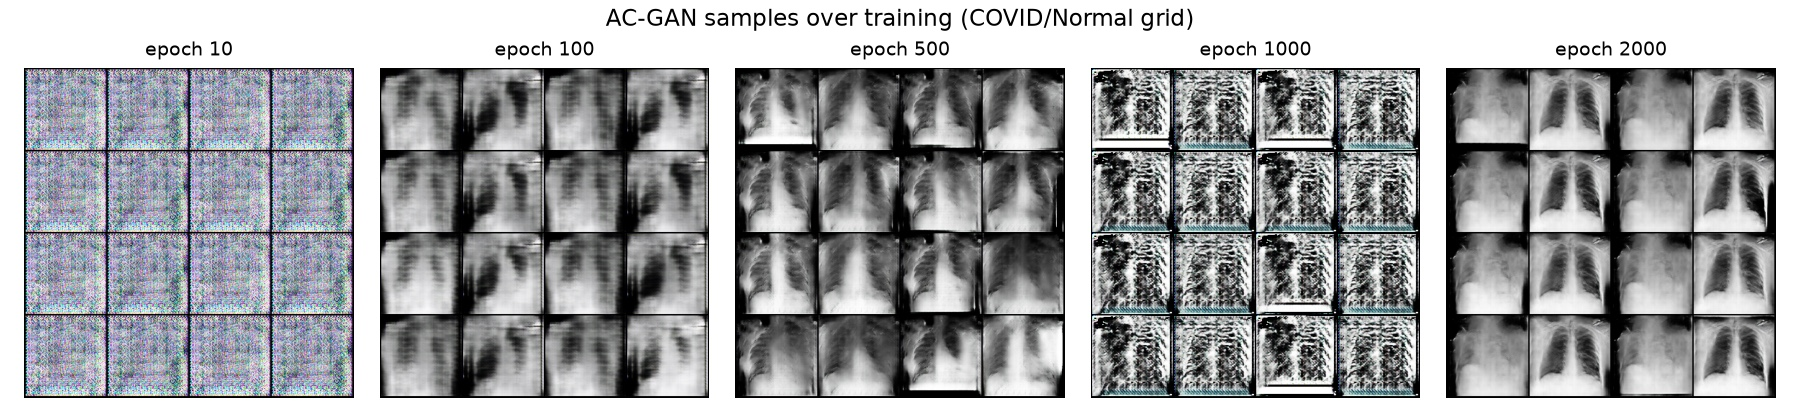
\includegraphics[width=0.70\linewidth]{gan_samples.jpg}
\caption{\textbf{The fingerprint, seen.} 2000-epoch AC-GAN samples: the COVID tiles
(columns~1 \& 3) are \emph{conspicuously brighter} than the darker, sharper Normal
tiles (columns~2 \& 4) --- a whole-image brightness difference anyone can spot at a
glance. On \emph{real} data class-mean brightness differs by only $\sim$3.5\%; the
GAN turned a faint tendency into a deterministic rule.}
\label{fig:samples}
\end{figure}

\paragraph{Real detail vs.\ fake fingerprint (no contradiction).} A separate check ---
blurring the \emph{real} images --- collapses accuracy and COVID recall, so the
classifier depends on \emph{fine} detail genuinely present in real X-rays. The fakes
lack exactly that fine detail (only the coarse brightness tag), so the two findings
\emph{agree} and jointly explain the flat result: the real task is won on fine
pathology, which the synthetic images do not supply.

\paragraph{Diagnosis $\rightarrow$ two fixes, and a second dataset.} Anomaly~B has two
blockers: a \textbf{fingerprinting GAN} and a \textbf{frozen classifier head} with no
capacity to use new data. §\ref{sec:improvedarch} fixes both. And because anomaly~A is
a hypothesis about \emph{our data}, we test it directly: if the reproduction failure
were an artifact of our cleaner COVID set, it should behave differently on a different
one. So we \textbf{re-run the entire pipeline on a second dataset of the same kind of
task} --- \textbf{CBIS-DDSM} benign-vs-malignant mammography (a static, versioned
benchmark; 1{,}318 train / 378 test ROIs; two data bugs fixed first --- mask
contamination and 16-bit grayscale truncation) --- and report DDSM alongside every
main claim below.

% =====================================================================
\section{Improved architecture}
\label{sec:improvedarch}
% =====================================================================
Stage~1 surfaced two bottlenecks, so we improve on two fronts (all drawn from the
assignment's allowed modifications):

\begin{itemize}[nosep,leftmargin=1.4em]
  \item \textbf{Track A --- the classifier (fix the frozen head).} Unfreeze the top
        VGG16 conv block(s) (trainable params 33K $\to$ 7.11M at uf=1 $\to$ 13.01M at
        uf=2) and add a \textbf{BatchNorm head}, trained with \textbf{discriminative
        learning rates} (head \code{1e-3}, backbone \code{1e-5}) so ImageNet filters
        adapt without being destroyed on $\sim$900 images.
  \item \textbf{Track B --- the generator (kill the fingerprint).} Raise the latent
        noise $z\sim\mathcal{N}(0,0.02)\to\mathcal{N}(0,1)$ (0.02 nearly switches the
        noise off, collapsing $G$ to one prototype per class); add \textbf{DiffAugment}
        + \textbf{spectral norm} (small-data stability); and replace the auxiliary
        class head with a \textbf{projection discriminator}, which removes the
        fingerprint incentive at its root.
\end{itemize}

\noindent The architecture (layer shapes, $\sim$22M~G / $\sim$2M~D) is otherwise
unchanged, so gains are attributable to the recipe, not a bigger model. On DDSM the
\emph{same two axes} are applied: the GAN improvement there is \textbf{spectral norm +
kernel~$5{\to}4$/stride~2} (a different recipe reaching the same goal), and the
identical unfreeze-the-encoder change.

% =====================================================================
\section{Improved results --- main claims (CovidGAN + DDSM)}
\label{sec:results}
% =====================================================================
Each claim states the CovidGAN result first, then the DDSM check on independent data.

\subsection{Claim 1 --- unfreezing the classifier raises the baseline \emph{and} revives augmentation}
CovidGAN, mean~$\pm$~std over \textbf{5 seeds} (paper/reconstruction are single runs):

\begin{table}[htbp]\centering\small
\begin{tabular}{@{}lccc@{}}\toprule
\textbf{Model} & \textbf{CNN-AD} & \textbf{CNN-SA} & \textbf{Lift} \\ \midrule
Paper (Waheed et al.) & 85.00\% & 95.00\% & +10.00 \\
Reconstruction (frozen) & 90.62\% & 90.10\% & $-$0.52 (flat) \\
Improved / uf=1 & 92.50\,$\pm$\,0.71 & 93.65\,$\pm$\,1.16 & \textbf{+1.15} \\
Improved / uf=2 & \textbf{94.48\,$\pm$\,0.97} & \textbf{96.67\,$\pm$\,0.71} & \textbf{+2.19} \\
\bottomrule\end{tabular}\end{table}

\noindent Unfreezing raised the baseline (90.6$\to$94.5\%) \emph{and} restored the
lift; at uf=2, \textbf{CNN-SA 96.67\% edges past the paper's 95\%} (COVID-recall lift
+3.33, larger than each arm's seed spread). \emph{Data-scarcity sweep:} the lift is
positive at every real-data fraction and largest in the low-to-mid regime (peak +3.30
at 25\% real), consistent with the paper's ``augmentation rescues data-starved
models'' reading and explaining why our full-data lift is $\sim$+2, not +10.

\paragraph{Second dataset (DDSM): holds.} Unfreezing raises the DDSM baseline
identically --- frozen AD 66.00\% $\to$ unfrozen AD 69.45\% (+3.45, both seeds) ---
and with the unfrozen classifier, baseline-GAN augmentation gives DDSM's first fully
reproducible augmentation win (70.77\% $>$ 69.45\% at both seeds). Capacity is the
precondition for augmentation to help, on both datasets.

\begin{figure}[htbp]\centering
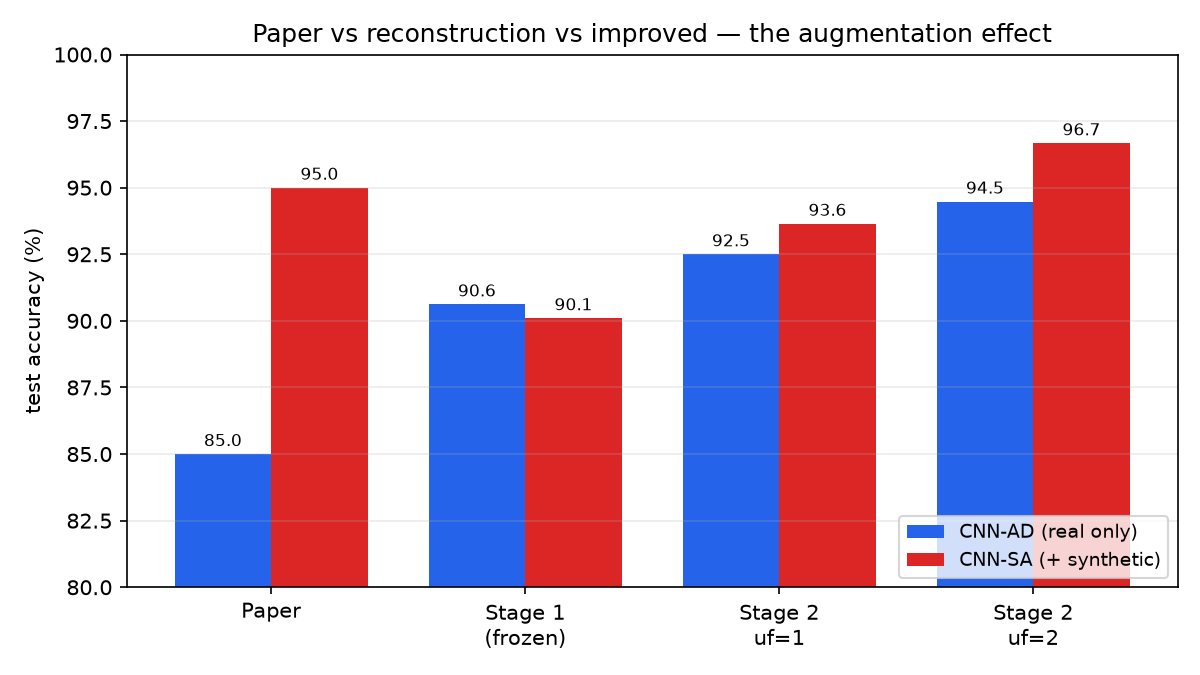
\includegraphics[width=0.80\linewidth]{comparison_bar.png}
\caption{Paper vs.\ reconstruction vs.\ improved (CovidGAN). Frozen Stage~1 shows no
augmentation gain; both improved variants raise the baseline and restore a positive
lift, uf=2 CNN-SA edging past the paper's 95\%.}
\end{figure}

\subsection{Claim 2 --- the improved GAN carries real transferable signal (not a fingerprint)}
CovidGAN generator quality vs.\ transfer probe (floor = 62.5\%):

\begin{table}[htbp]\centering\small
\begin{tabular}{@{}lcc@{}}\toprule
\textbf{Generator} & \textbf{FID} & \textbf{Transfer-probe acc.} \\ \midrule
Stage-1 AC-GAN, 2000 ep (noise 0.02) & 272.7 & \textbf{55.2\%} (below floor) \\
Improved AC-GAN, 300 ep & 225.7 & 72.9\% \\
Projection discriminator, 300 ep & 155.0 & 74.5\% \\
\textbf{Projection discriminator, 600 ep} & \textbf{121.3} & \textbf{81.3\%} \\
\bottomrule\end{tabular}\end{table}

\noindent Raising the noise to 1.0 is the biggest lever (55$\to$73\%); the projection
discriminator is the least-fingerprinted generator and at 300~ep already beats the
Stage-1 AC-GAN at 2000~ep by $\sim$43\% FID. \textbf{Second dataset (DDSM): holds ---}
the spectral-norm + kernel/stride GAN cut loss variance $\sim$10--30$\times$ and moved
synthetic malignant samples into overlap with the real-malignant PCA region (a
de-fingerprinted, more stable generator, reached via a different intervention).

\subsection{Claim 3 --- a better generator does not (necessarily) help the classifier}
This is the project's most surprising result. On CovidGAN, taking the projection pool
300$\to$600 epochs (FID 155$\to$121, transfer 74.5$\to$81.3\% --- better by \emph{every}
generator-side metric) moved downstream accuracy the \emph{wrong} way (single seed):

\begin{table}[htbp]\centering\small
\begin{tabular}{@{}lccc@{}}\toprule
\textbf{Classifier} & \textbf{AD} & \textbf{SA + Proj 300} & \textbf{SA + Proj 600} \\ \midrule
frozen          & 90.62\% & 90.10\% & \textbf{88.54\%} \\
unfrozen (uf=2) & 95.31\% & 97.40\% & \textbf{93.75\%} \\
\bottomrule\end{tabular}\end{table}

\noindent Lower FID \emph{and} higher transfer, yet downstream dropped ---
\textbf{GAN quality metrics do not predict downstream augmentation value.}
\ddsmonly{Second dataset (DDSM): the same reversal, established at \emph{two seeds}
with a mechanism probe --- the improved GAN helps at matched epochs but \emph{hurts}
the unfrozen classifier (66.67\% $<$ baseline-GAN 70.77\% and $<$ AD 69.45\%, both
seeds). This currently leads on DDSM: the CovidGAN reversal is only single-seed with
no mechanism probe, so a multi-seed CovidGAN run + a synthetic-only probe of the
projection 300-vs-600 pools still needs to be added.}

\subsection{Claim 4 --- both fixes are required (and the GAN gain needs capacity)}
CovidGAN \{improved AC-GAN, projection\} pool $\times$ \{frozen, unfrozen\} classifier
(single seed; the uf=2 lift itself is 5-seed confirmed at +2.19):

\begin{table}[htbp]\centering\small
\begin{tabular}{@{}lccc@{}}\toprule
\textbf{Classifier} & \textbf{AD} & \textbf{SA + AC-GAN} & \textbf{SA + Projection} \\ \midrule
frozen   & 90.62\% & 90.10\% & 90.10\% \\
unfrozen & 95.31\% & \textbf{97.92\%} & 97.40\% \\
\bottomrule\end{tabular}\end{table}

\noindent Better GANs help \textbf{only when the encoder is unfrozen}; under the
frozen head they stay flat, and with scarce real data they actively \emph{hurt} (acc
lift $-1.9$ at 100\% real $\to -8.2$ at 10\%). \textbf{Neither fix alone reproduces
the paper's benefit.} \textbf{Second dataset (DDSM): holds} --- the analogous
capacity~$\times$~GAN-source grid shows the same structure (flat under the frozen
head, a reproducible win only once unfrozen).

\medskip
\noindent\ddsmonly{DDSM-only, CovidGAN counterpart to add:} On DDSM, improving the
GAN architecture produced a clean \emph{downstream} gain at matched epochs
(baseline-GAN SA 60.05\% $\to$ improved-GAN SA 66.93\%, \textbf{+6.9}, vs.\ real-only
AD 64.02\%) --- a case where a generation-quality improvement \emph{did} translate
downstream, because that classifier is far from ceiling.
\ddsmonly{We do not yet have the matched CovidGAN experiment isolating an improved-GAN
downstream gain at equal epochs; it should be run and inserted here.} Likewise the
DDSM capacity grid and the Claim~3 reversal are at two seeds while CovidGAN's are
single-seed --- \ddsmonly{the CovidGAN grid needs re-running multi-seed
(\code{stage2/multiseed.py}) to match DDSM's power.}

% =====================================================================
\section{Discussion}
% =====================================================================
\paragraph{The failure is not an artifact of our COVID data.} The naive +10 setup
failed on \emph{both} datasets, and every CovidGAN conclusion we checked on DDSM held
on independent data. So the failure to reproduce is a property of the \emph{method
under these conditions}, not of our particular dataset. The paper's claim reproduces
\emph{in kind, not in magnitude}: +2.19 on COVID (uf=2), and on DDSM the first
reproducible win plus a +6.9 matched-epoch GAN gain.

\paragraph{Generation quality does not predict downstream benefit.} On COVID, FID
halved and the transfer probe rose 55$\to$81\% with zero-or-negative downstream
change; on DDSM a far more stable, better-aligned generator hurt the high-capacity
classifier. Both datasets independently produced the same reversal --- only an
AD-vs-SA comparison measures the paper's actual claim.

\paragraph{Two knobs govern whether augmentation helps.} \emph{Capacity}: unfreezing
the encoder raised the baseline on both datasets and is the precondition for any
augmentation gain. \emph{Headroom}: the +10 is a data-starved, low-baseline regime,
reproducible in kind but not in magnitude on data (either dataset) that is not
starved.

\paragraph{Limitations \& future work.} Close the CovidGAN gaps flagged in
\textcolor{red}{\textbf{red}} above (multi-seed the reversal and the capacity$\times$GAN
grid; add the matched improved-GAN downstream comparison); unify the improved-GAN
recipe across datasets and run one shared multi-seed grid; replicate the scarcity
sweep on DDSM; and validate on an independent public CXR set to fully settle
anomaly~A. Full derivations, all eight controlled tests, and reproduce commands are in
the long-form report and repo logs (\code{REPORT.md}, \code{SESSION_FINDINGS.md}).

% =====================================================================
\section*{References}
% =====================================================================
\begin{enumerate}[nosep,leftmargin=1.6em]
  \item A.~Waheed et al., ``CovidGAN: Data Augmentation Using Auxiliary Classifier GAN
        for Improved Covid-19 Detection,'' \emph{IEEE Access}, vol.~8, 2020.
  \item A.~Odena, C.~Olah, J.~Shlens, ``Conditional Image Synthesis with Auxiliary
        Classifier GANs,'' \emph{ICML}, 2017.
  \item T.~Miyato, M.~Koyama, ``cGANs with Projection Discriminator,'' \emph{ICLR}, 2018.
  \item T.~Miyato et al., ``Spectral Normalization for GANs,'' \emph{ICLR}, 2018.
  \item S.~Zhao et al., ``Differentiable Augmentation for Data-Efficient GAN Training,''
        \emph{NeurIPS}, 2020.
  \item A.~Odena, V.~Dumoulin, C.~Olah, ``Deconvolution and Checkerboard Artifacts,''
        \emph{Distill}, 2016.
  \item K.~Simonyan, A.~Zisserman, ``Very Deep Convolutional Networks'' (VGG16),
        \emph{ICLR}, 2015.
  \item M.~Heusel et al., ``GANs Trained by a Two Time-Scale Update Rule'' (FID),
        \emph{NeurIPS}, 2017.
  \item T.~Rahman, M.~E.~H.~Chowdhury et al., ``COVID-19 Radiography Database,'' Kaggle.
  \item R.~S.~Lee et al., ``A curated mammography data set'' (CBIS-DDSM),
        \emph{Scientific Data}, 2017.
\end{enumerate}

\end{document}
